\documentclass{article}

\usepackage{graphicx}

\begin{document}

\vspace*{3ex}
\begin{flushright}
{\large 3 March 2015}
\end{flushright}

\begin{flushleft}
{\large Jakub Ciecierski\\

}
\end{flushleft}

\hskip3cm

\begin{center}

\Large {\bf
	Cellular automaton
}

\Large {\bf 
	Requirement specification 
}

\vskip2ex


\end{center}

\vskip20ex

\newpage

\section{Goal} 
\Large
\hspace{15pt}The goal of this project is to create an application for cellular automaton. The application 
will allow user to create, save and edit rules and observe new generations on the grid of cells.

\section{Glossary} \par


\setlength{\parindent}{5ex}
\Large {\bf \hspace{15pt} Cellular automaton } - consists of a \textit{grid} of \textit{cells}, each in one of a finite number of \textit{states} (e.g. on and off). 
	A new \textit{generation} is created, according to some fixed
	\textit{rule} that determines the new state of each cell. \\


\Large {\bf 
	Cell 
}	
	- can be in one of many states,
	in case of binary cellular automaton we only have two states for each cell, namely on and off.
	For each cell, a set of cells called its
	\textit{neighborhood} is defined relative to that cell.	\\


\Large {\bf 
	Grid
} 	
	- can be in any finite number of dimensions. Consists of cells.
	An initial state is selected by assigning a state for each cell \\


\Large {\bf Rule
} 
	- determines the new state of each cell in terms of the current state
	of the cell and the states of the cells in its neighborhood.
	Typically, the rule for updating the state of cells is the same for each
	cell, and is applied to the whole grid simultaneously, such application of
	a rule to the entire grid, creates a new \textit{generation} \\

\newpage	

\Large {\bf Neighborhood
} 
	-  have possibility to introduce rules which determine the new state of 
	each cell. Defined under different environments such as:
	\begin{itemize}
	
	\item	
		4 points neighborhood \hspace{35pt} 
			 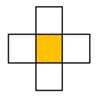
\includegraphics[width=20mm]{images/4_neigh.png} \\

	\item	
		8 points neighborhood \hspace{35pt}
			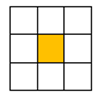
\includegraphics[width=20mm]{images/8_neigh.png} \\

	\item	
		24 points neighborhood \hspace{35pt}
			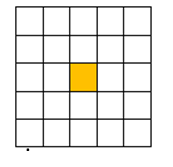
\includegraphics[width=20mm]{images/24_neigh.png} \\				
	\end{itemize}

\Large {\bf Pattern
} - is a combination of specific layout of cells on the grid and the set of rules to be applied for them.




\section{Description of requirements}

\hspace{15pt} The automaton will consist of binary set of states 
(e.i. on / off) and will operate in 3 different environments:
\begin{itemize}
	\item 4 points neighborhood.
	\item 8 points neighborhood.
	\item 24 points neighborhood.
\end{itemize}

\par The application will allow user to create, save and edit rules based on this environments and of course observe each generation on the two dimensional finite in size grid of cells
(the grid will have wrapping option to simulate infinite size - the left edge will be connected with right edge).

\par The user will be able to draw cells on the grid and save the state of grid into patterns.
The user can easily move around the grid, zoom in and out.


\section{User stories}
	Grid editor
\begin{itemize}	
	\item 
		As a user, 
		I want to open grid editor,
		in order to change the grid size.

	\item 
		As a user, 
		I want to open grid editor,
		in order to change color of each state of a cell.

	\item 
		As a user, 
		I want to open grid editor,
		in order to enable/disable wrapping option.

	\vspace{30pt}
	Rule editor
	
	\item 
		As a user,
		I want to open rule editor,
		in order to create new rule.
		
	\item 
		As a user,
		I want to choose neighborhood environment,
		in order to add new rule.
		
	\item 
		As a user,
		I want to define specific transition for a given state of cell,
		in order to generate new state.
		
	\item 
		As a user,
		I want to click save/save as button in rule editor,
		in order to save current rule.

	\item 
		As a user,
		I want to click load button in rule editor,
		in order to load current rule and possible edit it.

	\vspace{30pt}
	Application option
	
	\item 
		As a user,
		I want to move View components (e.g. rule editor / grid editor / browser),
		in order to position them in different location.
	\item 
		As a user,
		I want to click next generation button 
		to compute next generation
	\item 
		As a user,
		I want to click next N generations button,
		to compute next N generations.
	\item 
		As a user,
		I want to set the number of generation to skip by clicking next N generations button,
		in order to compute next N generations.
	\item 
		As a user,
		I want set the speed of computation of next generation in running mode,
		to customize the speed of which the automaton is transitioning.

\end{itemize}


\section{Requirements of specification}

\begin{itemize}
	\item A	
\end{itemize}

\section{GUI mock-up}

\section{Evaluation of solution}

\end{document}
